\documentclass{oblivoir}
%%%Default packages
\usepackage{amsmath,amssymb,amsthm,kotex,tabu,graphicx,pifont}
\usepackage{../kswrapfig}

\usepackage{gensymb} %\degree

%%%More packages
%\usepackage{caption,subcaption}
%\usepackage[perpage]{footmisc}
%
\usepackage[skipabove=10pt,innertopmargin=10pt,nobreak=true]{mdframed}

\usepackage[inline]{enumitem}
\setlist[enumerate,1]{label=(\arabic*)}
\setlist[enumerate,2]{label=(\alph*)}

\usepackage{multicol}
\setlength{\columnsep}{30pt}
\setlength{\columnseprule}{1pt}
%
%\usepackage{forest}
%\usetikzlibrary{shapes.geometric,arrows.meta,calc}
%
%%%defi theo exam prob rema proo
%이 환경들 아래에 문단을 쓸 경우 살짝 들여쓰기가 되므로 \hspace{-.7em}가 필요할 수 있다.

\newcounter{num}
\newcommand{\defi}[1]
{\noindent\refstepcounter{num}\textbf{정의 \arabic{num})} #1\par\noindent}
\newcommand{\theo}[1]
{\noindent\refstepcounter{num}\textbf{정리 \arabic{num})} #1\par\noindent}
\newcommand{\revi}[1]
{\noindent\refstepcounter{num}\textbf{복습 \arabic{num})} #1\par\noindent}
\newcommand{\exam}[1]
{\bigskip\bigskip\noindent\refstepcounter{num}\textbf{예시 \arabic{num})} #1\par\noindent}
\newcommand{\prob}[1]
{\bigskip\bigskip\noindent\refstepcounter{num}\textbf{문제 \arabic{num})} #1\par\noindent}
\newcommand{\rema}[1]
{\bigskip\bigskip\noindent\refstepcounter{num}\textbf{참고 \arabic{num})} #1\par\noindent}
\newcommand{\proo}
{\bigskip\noindent\textsf{증명)}}

\newenvironment{talign}
 {\let\displaystyle\textstyle\align}
 {\endalign}
\newenvironment{talign*}
 {\let\displaystyle\textstyle\csname align*\endcsname}
 {\endalign}
%
%%%Commands

\newcommand{\procedure}[1]{\begin{mdframed}\vspace{#1\textheight}\end{mdframed}}

\newcommand\an[1]{\par\bigskip\noindent\textbf{문제 \ref{#1})}\par\noindent}

\newcommand\ann[2]{\par\bigskip\noindent\textbf{문제 \ref{#1})}\:\:#2\par\medskip\noindent}

\newcommand\ans[1]{\begin{flushright}\textbf{답 : }#1\end{flushright}}

\newcommand\anssec[1]{\bigskip\bigskip\noindent{\large\bfseries#1}}

\newcommand{\pb}[1]%\Phantom + fBox
{\fbox{\phantom{\ensuremath{#1}}}}

\newcommand\ba{\,|\,}

\newcommand\ovv[1]{\ensuremath{\overline{#1}}}
\newcommand\ov[2]{\ensuremath{\overline{#1#2}}}
%
%%%% Settings
%\let\oldsection\section
%
%\renewcommand\section{\clearpage\oldsection}
%
%\let\emph\textsf
%
%\renewcommand{\arraystretch}{1.5}
%
%%%% Footnotes
%\makeatletter
%\def\@fnsymbol#1{\ensuremath{\ifcase#1\or
%*\or **\or ***\or
%\star\or\star\star\or\star\star\star\or
%\dagger\or\dagger\dagger\or\dagger\dagger\dagger
%\else\@ctrerr\fi}}
%
%\renewcommand{\thefootnote}{\fnsymbol{footnote}}
%\makeatother
%
%\makeatletter
%\AtBeginEnvironment{mdframed}{%
%\def\@fnsymbol#1{\ensuremath{\ifcase#1\or
%*\or **\or ***\or
%\star\or\star\star\or\star\star\star\or
%\dagger\or\dagger\dagger\or\dagger\dagger\dagger
%\else\@ctrerr\fi}}%
%}   
%\renewcommand\thempfootnote{\fnsymbol{mpfootnote}}
%\makeatother
%
%%% 객관식 선지
\newcommand\one{\ding{172}}
\newcommand\two{\ding{173}}
\newcommand\three{\ding{174}}
\newcommand\four{\ding{175}}
\newcommand\five{\ding{176}}
\usepackage{tabto,pifont}
%\TabPositions{0.2\textwidth,0.4\textwidth,0.6\textwidth,0.8\textwidth}

\newcommand\taba[5]{\par\noindent
\one\:{#1}
\tabto{0.2\textwidth}\two\:\:{#2}
\tabto{0.4\textwidth}\three\:\:{#3}
\tabto{0.6\textwidth}\four\:\:{#4}
\tabto{0.8\textwidth}\five\:\:{#5}}

\newcommand\tabb[5]{\par\noindent
\one\:{#1}
\tabto{0.33\textwidth}\two\:\:{#2}
\tabto{0.67\textwidth}\three\:\:{#3}\medskip\par\noindent
\four\:\:{#4}
\tabto{0.33\textwidth}\five\:\:{#5}}

\newcommand\tabc[5]{\par\noindent
\one\:{#1}
\tabto{0.5\textwidth}\two\:\:{#2}\medskip\par\noindent
\three\:\:{#3}
\tabto{0.5\textwidth}\four\:\:{#4}\medskip\par\noindent
\five\:\:{#5}}

\newcommand\tabd[5]{\par\noindent
\one\:{#1}\medskip\par\noindent
\two\:\:{#2}\medskip\par\noindent
\three\:\:{#3}\medskip\par\noindent
\four\:\:{#4}\medskip\par\noindent
\five\:\:{#5}}
%
%%%% fonts
%
%\usepackage{fontspec, xunicode, xltxtra}
%\setmainfont[]{은 바탕}
%\setsansfont[]{은 돋움}
%\setmonofont[]{은 바탕}
%\XeTeXlinebreaklocale "ko"
%%%%
\begin{document}

\title{수학(하) : 12 경우의 수}
\author{}
\date{\today}
\maketitle
\tableofcontents
\newpage


%%
\section{합의 법칙과 곱의 법칙}
\begin{minipage}{.8\textwidth}\label{law1}
%
\exam{주사위를 한 번 던질 때, 나온 눈의 수가 짝수이거나\\ 5의 약수인 경우의 수를 구해보자.}
\end{minipage}
\begin{minipage}{.2\textwidth}
\centering
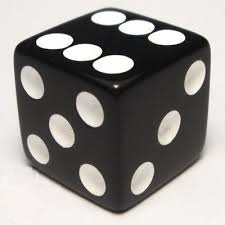
\includegraphics[width=.5\textwidth]{dice1}
\end{minipage}
\begin{mdframed}
주사위의 눈이 짝수인 경우는 2, 4, 6의 세 가지이고
5의 약수인 경우는 1, 5의 두 가지이다.
두 경우가 서로 겹치지 않으므로 주사위의 눈이 짝수이거나 5의 약수인 경우의 수는 \(3+2=5\)의 다섯 가지이다.
\end{mdframed}
\ans{5}

\bigskip
짝수가 나오는 사건을 \(A\), 5의 약수가 나오는 사건을 \(B\)라고 하자.
\(A\)와 \(B\)를 집합처럼 생각하면
\[A=\{2,4,6\},\quad B=\{1,5\}\]
이다.
이때 \(A\cap B\neq\varnothing\)이므로
\[n(A\cup B)=n(A)+n(B)\]
로 계산할 수 있는 것이다.

%3의 배수는 3, 6, 9, 12의 네 개이고 5의 배수는 5, 10의 두 개이다.
%두 경우는 겹치는 경우가 없으므로 3 또는 5의 배수가 나오는 경우의 수는 4+2=6개이다.

%%
%\exam{}
%\begin{minipage}{.6\textwidth}\label{law1}
%각 면에 1부터 12까지의 자연수가 적혀 있는 정십이면체 주사위를 한 번 던져 윗면에 적힌 수를 관찰하자.
%오른쪽 그림은 숫자 2가 나온 경우이다.
%이때 %다음을 구하여라.
%주사위의 눈이
%3 또는 5의 배수가 나오는 경우의 수를 구해보자.
%\end{minipage}
%\begin{minipage}{.4\textwidth}
%\centering
%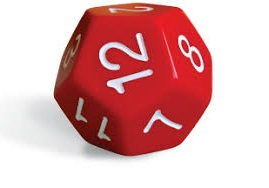
\includegraphics[width=\textwidth]{dodecahedron}
%\end{minipage}
%
%3의 배수는 3, 6, 9, 12의 네 개이고 5의 배수는 5, 10의 두 개이다.
%두 경우는 겹치는 경우가 없으므로 3 또는 5의 배수가 나오는 경우의 수는 4+2=6개이다.

\begin{mdframed}
%
\theo{합의 법칙}\label{law2}
\hspace{-.7em}
두 사건 \(A\), \(B\)가 일어나는 경우의 수가 각각 \(m\), \(n\)이고 두 사건 \(A\), \(B\)가 동시에 일어나지 않을 때, 사건 \(A\) 또는 사건 \(B\)가 일어나는 경우의 수는 \(m+n\)이다.
\end{mdframed}

%
\prob{}\label{law3}
\hspace{-.7em}
수빈이는 친구의 생일 선물로 줄 책을 한 권 고르려고 한다.
서로 다른 시집 5권과 서로 다른 수필집 4권 중에서 한 권을 고르는 경우의 수를 구하여라.
\newpage

\noindent
\begin{minipage}{.8\textwidth}\label{law4}
%
\exam{주사위를 두 번 던질 때, 첫 번째 눈의 수가 짝수이고 두 번째 눈의 수는 5의 약수인 경우의 수를 구해보자.}
\end{minipage}
\begin{minipage}{.2\textwidth}
\centering
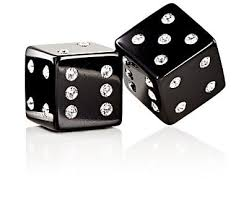
\includegraphics[width=.9\textwidth]{dice2}
\end{minipage}
\begin{mdframed}
%첫 번째 눈의 수는 2, 4, 6의 세 개의 수가 가능하고, 두 번째 눈의 수는 1, 5의 두 개의 수가 가능하다.
따라서 가능한 모든 경우를 수형도로 나타내면
\begin{center}
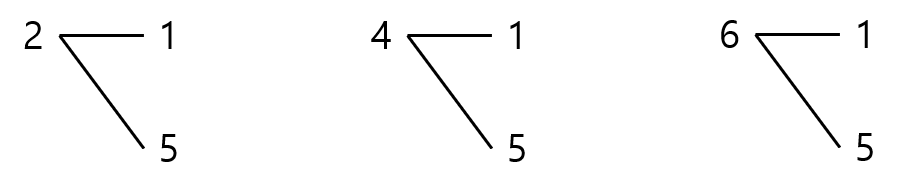
\includegraphics[width=.5\textwidth]{law_4}
\end{center}
이다.
따라서 가능한 경우의 수는 여섯 가지이다.
%첫 번째 주사위에서는 두 가지를 정할 수 있고
%두 번째 주사위에서는 세 가지를 정할 수 있으므로
이것은 \(3\times2=6\)으로 계산했다고 생각할 수도 있다.
\end{mdframed}
\ans{6}

\bigskip
문제에서 말하는 여섯 가지 경우의 수를 순서쌍으로 나타내면
\begin{gather*}
(2,1),(2,5),\\
(4,1),(4,5),\\
(6,1),(6,5)
\end{gather*}
%\begin{center}
%\begin{tabu}{c|ccc}
%	&2		&4		&6\\\hline
%1	&(2,1)	&(4,1)	&(6,1)\\
%5	&(2,5)	&(4,5)	&(6,5)
%\end{tabu}
%\end{center}
이다.
이 순서쌍들로 이루어진 집합 \(A\times B=\{(a,b)\ba a\in A,\;\;b\in B\}\)을 생각할 때,
\[n(A\times B)=n(A)\times n(B)\]
로 계산할 수 있는 것이다.
%\[A=\{2,4,6\},\quad B=\{1,5\}\]
%에서 문제에서 말하는 경우의 수는
%\begin{align*}
%A\times B
%&=\{(a,b)\ba a\in A,\;\;b\in B\}\\
%&=\{(2,1),(2,5),(4,1),(4,5),(6,1),(6,5)\}
%\end{align*}
%로 생각할 수 있으므로
%%\[A\times B=\{(2,1),(2,5),(4,1),(4,5),(6,1),(6,5)\}\]
%%이므로
%\[n(A\times B)=n(A)\times n(B)\]
%로 계산할 수 있는 것이다.

\begin{mdframed}
%
\theo{곱의 법칙}\label{law5}
\hspace{-.7em}
사건 \(A\)가 일어나는 경우의 수가 \(m\)이고, 그 각각의 경우에 대해 사건 \(B\)가 일어나는 경우의 수가 \(n\)일 때, 사건 \(A\)에 잇달아 사건 \(B\)가 일어나는 경우의 수는 \(m\times n\)이다.
%두 사건 \(A\), \(B\)가 일어나는 경우의 수가 각각 \(m\), \(n\)이고 두 사건 \(A\), \(B\)가 동시에 일어나지 않을 때, 사건 \(A\) 또는 사건 \(B\)가 일어나는 경우의 수는 \(m+n\)이다.
\end{mdframed}

%
\prob{}\label{law6}
\hspace{-.7em}
진우가 다니고 있는 학교에서는 과학 4과목, 사회 5과목을 가르친다.\\
과학 과목과 사회 과목 중 한 과목씩 택하여 공부하는 경우의 수를 구하여라.

\newpage
%
\prob{진헌이와 한솔이는 각각 중식점과 양식점에서 식사하려고 한다.}\label{law7}
\begin{center}
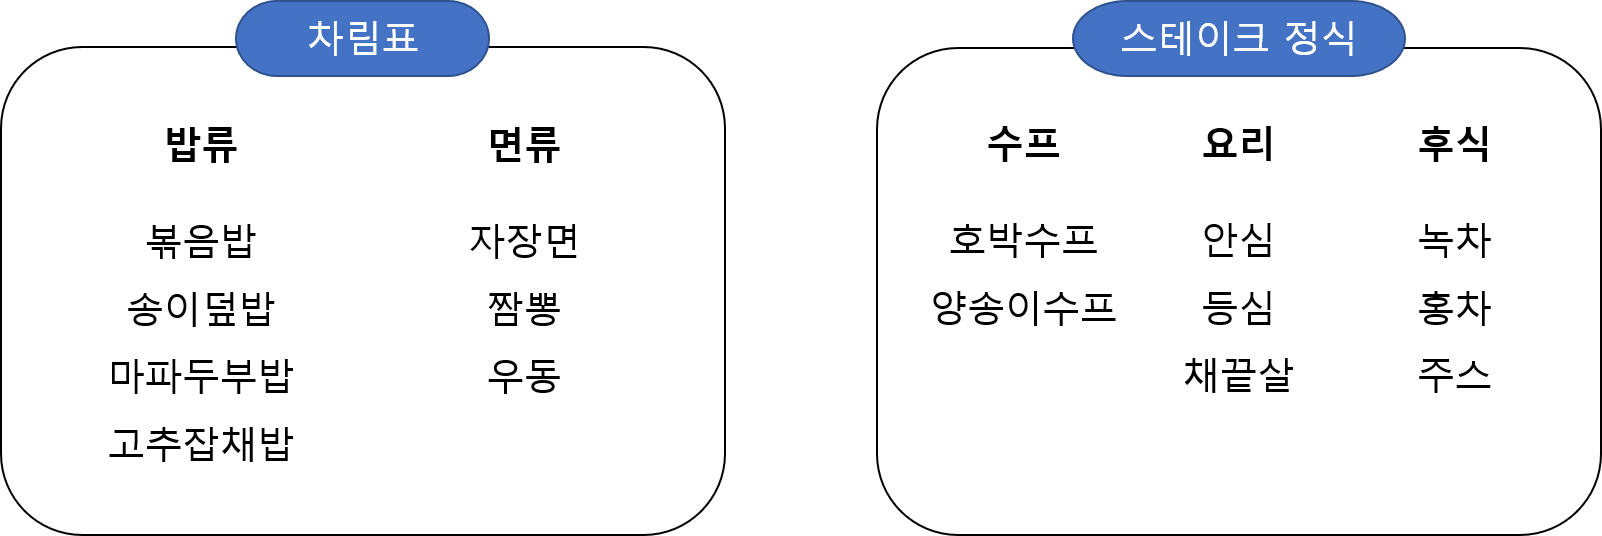
\includegraphics[width=.7\textwidth]{law_7}
\end{center}
진헌이는 밥류와 면류 중 하나만을 주문하고, 한솔이는 수프와 요리와 후식 중 하나씩을 주문하려고 한다.
두 사람이 각각 주문하는 경우의 수를 구하여라.

%
\prob{}\label{law8}
10원짜리 동전이 3개, 100원짜리 동전이 2개, 500원짜리 동전이 1개 있을 때, 이들 전부 또는 일부를 사용하여 지급할 수 있는 금액의 경우의 수는?
%만 원짜리 지폐 5장, 천 원짜리 지폐 7장, 백 원짜리 동전 3개로 지불할 수 있는 금액의 경우의 수는?
%(단, 0원을 지불하는 경우는 제외한다.)
\taba{22}{23}{24}{25}{26}

%
\prob{다음 식을 전개하였을 때 나타나는 모든 항의 개수를 구하시오.}
\begin{enumerate}\label{law9}
\item
\((a+b+c)(x+y+z)\)
\item
\((a+b+c+d)(x+y)\)
\end{enumerate}

%
\prob{}\label{law10}
정의역이 \(X=\{1,2,3,4\}\), 공역이 \(Y=\{a,b,c\}\)인 함수 \(f:X\to Y\)의 개수를 구하여라.
\begin{center}
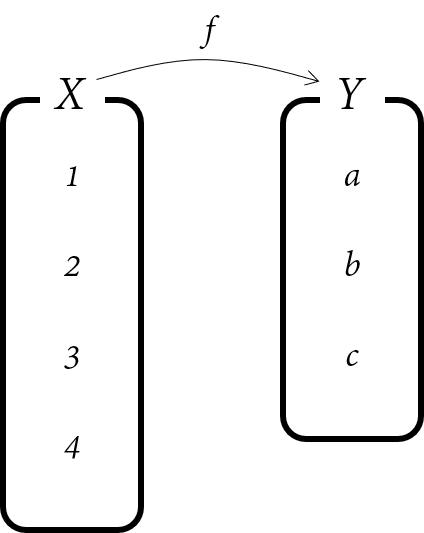
\includegraphics[width=.2\textwidth]{law_10}
\end{center}

\newpage
%
\exam{}
\begin{enumerate}\label{law11}
\item
12의 약수의 개수를 구하여라.
\item
12의 약수들의 합을 구하여라.
\end{enumerate}
\begin{mdframed}
12의 약수는 1, 2, 3, 4, 6, 12이다.
따라서 12의 약수의 개수는 여섯 개이고, 12의 약수들의 합은 \(1+2+3+4+6+12=28\)이다.
\end{mdframed}
\ans{(1)\; 6,\quad(2)\;28}

이 문제를 소인수분해를 통해 접근해보자.
12를 소인수분해하면 \(12=2^2\times3\)이다.
따라서 12의 소수들은 다음과 같이 표로 표현할 수 있다.
\begin{center}
\begin{tabu}to.4\textwidth{X[c,$]|X[c,$]X[c,$]}
\times	&1	&3^1\\\hline
1		&1	&3^1\\
2^1		&2^1	&2^1\times3^1\\
2^2		&2^2	&2^2\times3^1
\end{tabu}
\end{center}
%12의 약수는 \(2^m\times3^n\)의 꼴이며, 이때 \(0\le m\le2\), \(0\le n\le1\)이다.\footnotemark\\
%예를 들어 6은 12의 약수이며 이때 \(m=1\), \(n=1\)이다.
%
그러므로 12의 약수는 \(3\times2=6\)의 여섯 개이다.
12의 약수들의 합을 계산할 때에도 위의 표를 참고하면 다음 계산을 할 수 있다.
\begin{align*}
1+3^1+2^1+2^1\times3^1+2^2+2^2\times3^1
&=(1+3^1)+2^1(1+3^1)+2^2(1+3^1)\\
&=(1+3^1)(1+2^1+2^2)\\
&=4\cdot7=28
\end{align*}

%
\prob{54의 약수의 개수와 약수들의 합을 구하여라.}\label{law12}

%
\prob{60의 약수의 개수와 약수들의 합을 구하여라.}\label{law13}

%%
\section{순열}
%
\exam{네 개의 곡 \(a\), \(b\), \(c\), \(d\) 중 두 개의 곡을 차례대로 재생하는 방법의 수를 구하여라.}\label{perm1}
\begin{mdframed}
모든 경우의 수를 수형도로 나타내면,
\begin{center}
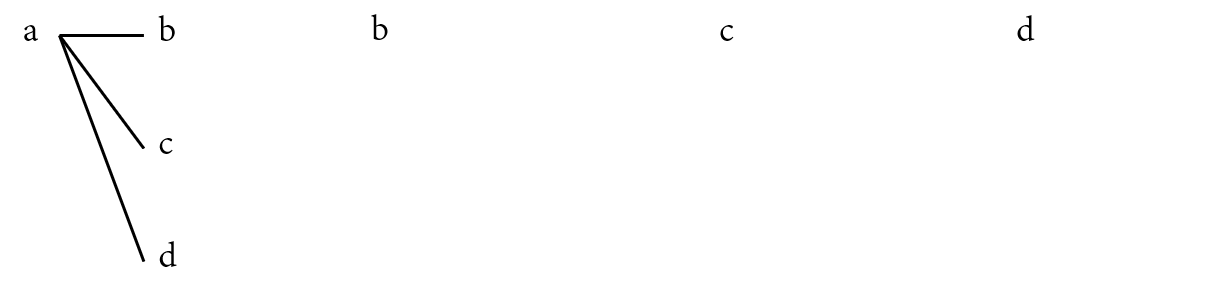
\includegraphics[width=.9\textwidth]{perm_1}
\end{center}
이다.
첫 번째로 재생할 수 있는 곡은 \(a\), \(b\), \(c\), \(d\)의 4가지이고, 각각에 대하여 두 번째로 재생할 수 있는 곡은 첫  번째로 재생한 곡을 제외한 3가지이다.
따라서, 곱의 법칙에 의하여 두 곡을 차례대로 재생하는 방법의 수는
\[4\times3=12\]
이다.
\end{mdframed}

%
\prob{}\label{perm2}
다섯 개의 곡 \(a\), \(b\), \(c\), \(d\), \(e\) 중 의 세 개의 곡을 차례대로 재생하는 방법의 수를 구하여라.

\newpage
예시 \ref{perm1})의 경우의 수를 기호로 \fbox{\(_4P_2\)}와 같이 나타낸다.
4개 중에서 2개를 택해 일렬로 나열하는 방법의 수이다.
한편, 문제 \ref{perm2})의 경우의 수는 \(\pb{_5P_3}\)으로 나타낼 수 있을 것이다.
\begin{mdframed}
%
\defi{순열}\label{perm3}
\hspace{-.7em}
서로 다른 \(n\)개에서 \(r\)개를 택하여 일렬로 나열하는 경우의 수를 \(_nP_r\)로 나타낸다.
\[_nP_r=n(n-1)(n-2)\cdots(n-r+1)\qquad(1\le r\le n)\]
\end{mdframed}

%
\prob{다음 값을 구하시오}\label{perm4}
(1)\;\;\(_3P_2\)\hspace{0.17\textwidth}
(2)\;\;\(_6P_3\)\hspace{0.17\textwidth}
(3)\;\;\(_4P_4\)\hspace{0.17\textwidth}
(4)\;\;\(_4P_1\)

%
\prob{연극에 참가할 9명 중에서 4개의 배역 \(A\), \(B\), \(C\), \(D\)를 정하는 경우의 수를 구하시오.}\label{perm5}

%
\prob{}\label{perm6}
다섯 개의 수 1, 2, 3, 4, 5,에서 서로 다른 세 개의 숫자를 택하여 세 자리 수를 만든다.
예를 들어 1, 5, 2를 택하여 세 자리 수 152를 만들 수 있다.
이렇게 만들 수 있는 세 자리 수의 개수를 구하시오.

%
\prob{}\label{perm7}
정의역이 \(X=\{1,2,3\}\), 공역이 \(Y=\{a,b,c,d\}\)인 일대일함수 \(f:X\to Y\)의 개수를 구하여라.
\begin{center}
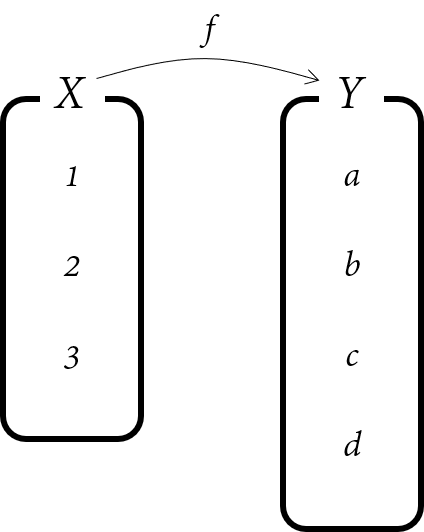
\includegraphics[width=.2\textwidth]{perm_7}
\end{center}


\newpage
\begin{mdframed}
%
\defi{\(n\)의 계승}\label{perm8}
\hspace{-.7em}
\[n!=n\times(n-1)\times(n-2)\times\cdots\times3\times2\times1\]
\end{mdframed}

%
\rema{}
\begin{enumerate}\label{perm9}
\item
\(!\)는 팩토리얼(factorial)이라고 읽는다.
%따라서 \(5!\)는 `\(5\) 팩토리얼'이다.
\item
\(5!=5\times4\times3\times2\times1=120\)
\item
\(0!=1\)로 정의한다.
\end{enumerate}

\bigskip
\(n!\)은 \(_nP_n\)과 같다.
즉 서로 다른 \(n\)개를 일렬로 나열하는 방법의 수이다.
%
\prob{}\label{perm10}
수빈이는 내일까지 수학 문제 풀기, 영어 단어 외우기, 역사 보고서 쓰기의 세 가지 숙제를 해야 한다.
한 번에 여러 개의 숙제를 할 수 없을 때 숙제의 순서를 정하는 방법의 수를 구하여라.

%
\prob{}\label{perm11}
우석, 유진, 찬희, 종원, 승미의 다섯 명의 학생이 100m 달리기에 참여한다.
순위가 정해지는 경우의 수를 구하여라.

\noindent
\begin{minipage}{0.7\textwidth}
%
\prob{}\label{perm12}
오른쪽 그림과 같은 영역에 빨강, 노랑, 초록, 파랑의 네 가지 색을 하나씩 칠할 때, 칠하는 방법의 수를 구하여라.
\end{minipage}
\begin{minipage}{0.25\textwidth}
\centering
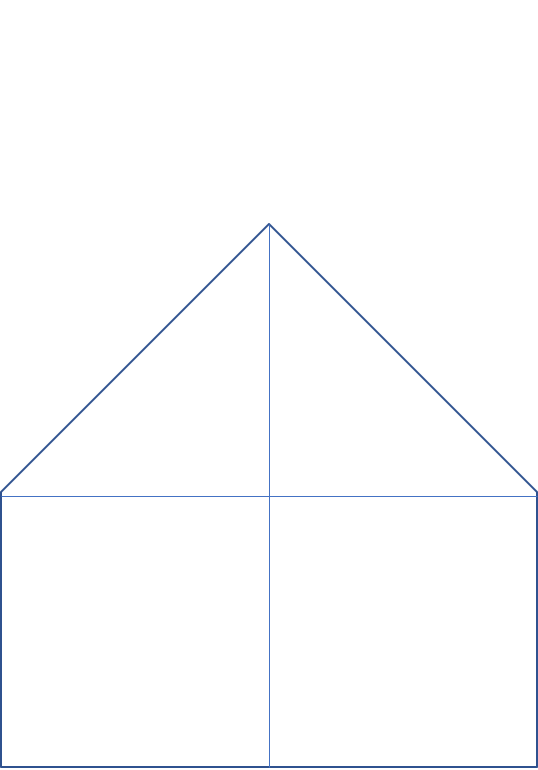
\includegraphics[width=.8\textwidth]{perm_12}
\end{minipage}

\newpage
팩토리얼을 사용하면 순열의 수를 깔끔한 형태로 쓸 수 있다.
\begin{mdframed}
%
\theo{}\label{perm13}
\[_nP_r=\frac{n!}{(n-r)!}\]
\end{mdframed}
예를 들어 \(_8P_3\)은
\[_8P_3=8\times7\times6\]
인데, 이것은
\[_8P_3=\frac{8!}{(8-3)!}=\frac{8\times7\times6\times5\times4\times3\times2\times1}{5\times4\times3\times2\times1}\]
로 계산한 결과와 같다.

%
\prob{정리 \ref{perm13})을 사용하여 다음을 계산하여라.}\label{perm14}
(1)\;\;\(_5P_2\)\hspace{0.26\textwidth}
(2)\;\;\(_3P_3\)\hspace{0.26\textwidth}
(3)\;\;\(_4P_0\)

%
\prob{다음 \(\pb{11}\)안에 알맞은 수를 써넣으시오}\label{perm15}
\\[5pt]
\begin{enumerate*}[itemjoin=\tabto{0.5\textwidth}]
\item
\(\displaystyle_{11}P_4=\frac{11!}{\pb{7}!}\)
\item
\(\displaystyle_{10}P_\square=\frac{10!}{7!}\)
\end{enumerate*}
%(1)\;\;\(\displaystyle_{11}P_4=\frac{11!}{\pb{7}!}\)\hspace{0.43\textwidth}
%(2)\;\;\(\displaystyle_{10}P_{\pb{4}}=\frac{10!}{7!}\)


%%
\section{조합}
%
\exam{네 개의 곡 \(a\), \(b\), \(c\), \(d\) 중 좋아하는 두 곡을 고르는 방법의 수를 구하여라.}\label{comb1}
\begin{mdframed}
두 개의 곡을 고르는 방법은
\[ab/ac/ad/bc/bd/cd\]
의 6가지이다.
따라서 예시 \ref{perm1})에서 구했던, 두 곡을 차례로 재생하는 방법의 수인  \(_4P_2=12\)와는 다르다.
예시 \ref{perm1})에서의 12가지 경우는
%예시 \ref{perm1})에서의 12가지인
\[ab/ac/ad/ba/bc/bd/ca/cb/cd/da/db/dc\]
이었다.
이때, 따라서 \(ab\)와 \(ba\)는 서로 다른 경우로 취급했었다.
\(a\)를 먼저 재생하고 \(b\)를 나중에 재생하는 것과 \(b\)를 먼저 재생하고 \(a\)를 나중에 재생하는 것을 구분해야 했기 때문이다.
하지만 지금처럼 두 개의 곡을 고르는 경우에는 \(ab\)와 \(ba\)가 서로 같은  경우를 나타낸다.

이처럼 12가지의 모든 경우가 한 쌍씩 같다.
\begin{gather*}
ab=ba,\quad ac=ca,\quad ad=da,\\
bc=cb,\quad bd=db,\quad cd=dc
\end{gather*}
따라서 \(_4P_2\)을 2로 나눈 값이 답이 될 것이다.
\[\frac{_4P_2}{2}=\frac{12}2=6\]
\end{mdframed}

%
\prob{여섯 개의 곡 \(a\), \(b\), \(c\), \(d\), \(e\), \(f\) 중 좋아하는 두 곡을 고르는 방법의 수를 구하여라.}\label{comb2}

%
\prob{다섯 개의 곡 \(a\), \(b\), \(c\), \(d\), \(e\) 중 좋아하는 세 곡을 고르는 방법의 수를 구하여라.}\label{comb3}

\bigskip\bigskip
예시 \ref{comb1})의 경우의 수를 기호로 \fbox{\(_4C_2\)}와 같이 나타낸다.
4개 중에서 2개를 선택하는 방법의 수이다.
한편, 
문제 \ref{comb2})의 경우의 수는 \(\pb{_6C_2}\)으로,
문제 \ref{comb3})의 경우의 수는 \(\pb{_5C_3}\)으로 나타낼 수 있을 것이다.

\begin{mdframed}
%
\defi{조합}\label{comb4}
\hspace{-.7em}
서로 다른 \(n\)개에서 \(r\)개를 선택하는 경우의 수를 \(_nC_r\)로 나타낸다.
\[_nC_r=\frac{_nP_r}{r!}\qquad(1\le r\le n)\]
\end{mdframed}

%
\prob{}\label{comb5}
9명의 탁구선수 중에서 시합에 나가는 3명의 대표 선수를 선발하는 경우의 수를 구하여라.

%
\prob{아래 그림과 같이 원 위에 6개의 점들이 있다. 다음을 구하여라.}
\begin{enumerate}\label{comb6}
\item
두 개의 점을 연결하여 만들 수 있는 선분의 개수
\item
세 개의 점을 연결하여 만들 수 있는 삼각형의 개수
\end{enumerate}
\begin{center}
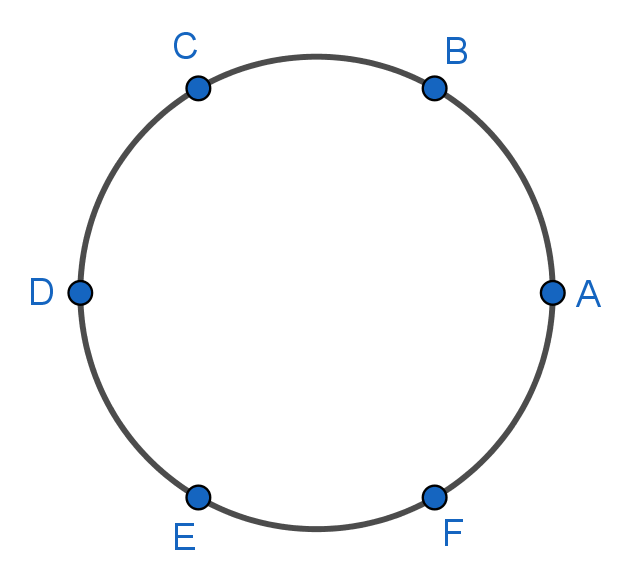
\includegraphics[width=.2\textwidth]{comb_6}
\end{center}

%
\prob{집합 \(A=\{a,b,c,d\}\)에 대하여}
\begin{enumerate}\label{comb7}
\item
\(A\)의 부분집합의 개수를 구하여라.
\item
\(A\)의 부분집합 중 원소의 개수가 2개인 부분집합의 개수를 구하여라.
\end{enumerate}

\newpage
순열에 관한 두 식
\begin{align*}
_nP_r&=n(n-1)(n-2)\cdots(n-r+1)\\
_nP_r&=\frac{n!}{(n-r)!}
\end{align*}
을 \(_nC_r=\frac{_nP_r}{r!}\)
에 각각 적용하면, 다음 공식들을 얻을 수 있다.
%순열 \(_nP_r\)의 식들을 이용하여, 다음 공식들을 사용할 수도 있다.
\begin{align}
_nC_r&=\frac{n(n-1)(n-2)\cdots(n-r+1)}{r!}\\
_nC_r&=\frac{n!}{r!(n-r)!}
\end{align}

%
\exam{}\label{comb8}
예를 들어 \(_{10}C_3\)를 계산할 때에는 (1)의 식을 사용해
\[_{10}C_3=\frac{10\times9\times8}{3\times2\times1}=120\]
로 계산해도 되고 (2)의 식을 사용해
\[_{10}C_3=\frac{10!}{7!3!}=\frac{10\times9\times8\times7\times6\times5\times4\times3\times2\times1}
{\left(7\times6\times5\times4\times3\times2\times1\right)\times\left(3\times2\times1\right)}=120\]
로 계산해도 된다.
약분과정에서 보듯 사실상 같은 계산이다.

\bigskip
실제 조합에 관한 계산에서는 (1)이 많이 쓰이고, 조합에 관한 증명을 할 때에는 (2)가 많이 쓰인다.

\bigskip
%
\prob{다음 조합의 수들을 계산하여라.}\label{comb9}\\
%\hspace{-.4em}
(1)\;\;\(_7C_0\)\hspace{0.2\textwidth}
(2)\;\;\(_7C_1\)\hspace{0.2\textwidth}
(3)\;\;\(_7C_2\)\hspace{0.2\textwidth}
(4)\;\;\(_7C_3\)\hspace{0.2\textwidth}\\[10pt]
(5)\;\;\(_7C_4\)\hspace{0.2\textwidth}
(6)\;\;\(_7C_5\)\hspace{0.2\textwidth}
(7)\;\;\(_7C_6\)\hspace{0.2\textwidth}
(8)\;\;\(_7C_7\)

\newpage
\mbox{}
\newpage
%%
\section*{답}
\addcontentsline{toc}{chapter}{\protect\numberline{*}답}
\begin{multicols*}{2}
%
\ann{law3}{9}

%
\ann{law6}{20}

%
\an{law7}
진헌 : 7, 한솔 : 18

%
\ann{law8}{\two}

%
\an{law9}
\begin{enumerate}
\item
9
\item
8
\end{enumerate}

%
\ann{law10}{81}

%
\an{law12}\\[-10pt]
\parbox{0.8\textwidth}{약수의 개수 : 8\\
약수들의 합 : 120}

%
\an{law13}\\[-10pt]
약수의 개수 : 12\\
약수들의 합 : 168
%약수의 개수 : 12, 약수들의 합 : 168

%
\ann{perm2}{60}

\columnbreak

%
\an{perm4}
\begin{enumerate}
\item
6
\item
120
\item
24
\item
4
\end{enumerate}

%
\ann{perm5}{3024}

%
\ann{perm6}{60}

%
\ann{perm7}{24}

%
\ann{perm10}{6}

%
\ann{perm11}{120}

%
\ann{perm12}{24}

%
\an{perm14}
\begin{enumerate}
\item
20
\item
6
\item
1
\end{enumerate}

\columnbreak
%
\an{perm15}
\begin{enumerate}%[itemjoin=\qquad\qquad]
\item
7
\item
3
\end{enumerate}

%
\ann{comb2}{15}

%
\ann{comb3}{10}

%
\ann{comb5}{84}

%
\an{comb6}
\begin{enumerate}
\item
15
\item
20
\end{enumerate}

%
\an{comb7}
\begin{enumerate}
\item
16
\item
6
\end{enumerate}

%
\an{comb9}
\begin{enumerate}
\item
1
\item
7
\item
21
\item
35
\item
35
\item
21
\item
7
\item
1
\end{enumerate}
\end{multicols*}

%%
\section*{요약}
\addcontentsline{toc}{chapter}{\protect\numberline{*}요약}
\begin{enumerate}[label=\arabic*.,itemsep=40pt]
\item
사건 \(A\), \(B\)가 일어나는 경우의 수가 각각 \(m\), \(n\)일 때,
\begin{enumerate}
\item
\(A\) 또는 \(B\)가 일어나는 경우의 수는 \(m+n\).
\item
\(A\)에 잇달아 \(B\)가 일어나는 경우의 수는 \(m\times n\).
\end{enumerate}
\item
순열\\[10pt]
서로 다른 \(n\)개에서 \(r\)개를 택하여 일렬로 나열하는 방법의 수는
\begin{align*}
_nP_r
&=n(n-1)(n-2)\cdots(n-r+1)\\
&=\frac{n!}{(n-r)!}
\end{align*}
\item
조합\\[10pt]
서로 다른 \(n\)개에서 \(r\)개를 선택하는 방법의 수는
\begin{align*}
_nC_r
&=\frac{_nP_r}{r!}\\
&=\frac{n(n-1)(n-2)\cdots(n-r+1)}{r!}\\
&=\frac{n!}{r!(n-r)!}
\end{align*}
\end{enumerate}

\end{document}